\chapter{Geração do mapa}

A posição do robô no mapa em cada instante é representada por um ponto no plano cartesiano e por um ângulo, que indica para qual sentido o robô está orientado. Esse ponto no plano indica onde está o centro de movimento do robô, que é o ponto médio entre as duas rodas.

Neste projeto, a determinação do deslocamento do robô é determinada primariamente pelos encoders presentes cada roda. O acelerômetro e o giroscópio são utilizados para aumentar a confiabilidade dos cálculos de deslocamento, principalmente em caso de escorregamento das rodas.

Na próxima seção será explicada a teoria da determinação do deslocamento, velocidade e aceleração do centro de movimento do robô a partir das leituras dos encoders em cada instante. Na seção \ref{sec:teoria_acel_giro} será explicitada a forma como as leituras do acelerômetro e giroscópio serão utilizadas para aumentar a confiabilidade das medições.

Na Figura \ref{fig:robo} está presente um esquema básico do robô visto de cima e virado com a frente para a direita. Nessa figura estão presentes os nomes das variáveis que são utilizadas nos cálculos posteriores.

\begin{figure}[H]
  \centering
  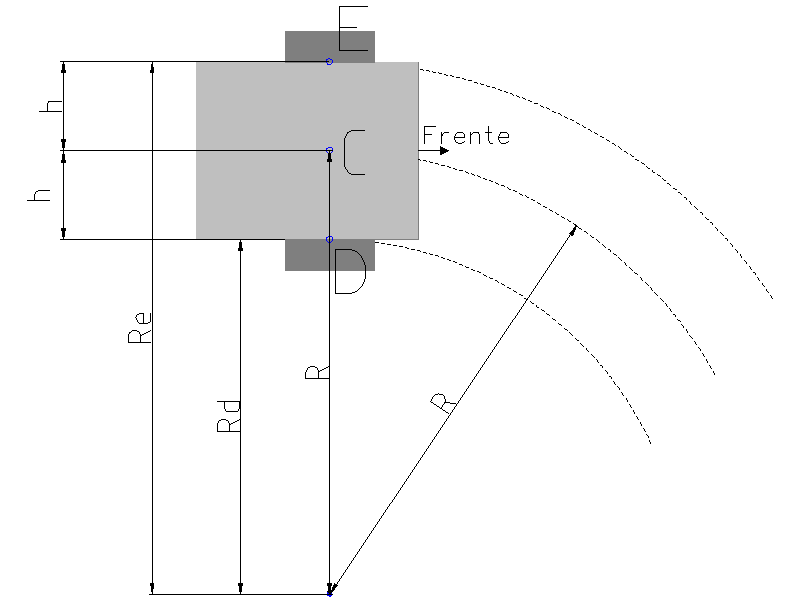
\includegraphics[width=0.5\textwidth, keepaspectratio]{./figuras/robo/robo.png}
  \caption{Representação básica do robô (visão superior).}
  \label{fig:robo}
\end{figure}

\section{Encoders}

Há dois dados importantes a determinar sobre o deslocamento do centro de movimento do robô: o deslocamento linear (distância absoluta percorrida) e o angular (variação do ângulo de orientação do robô). Cada encoder fornece uma medida de contagem de pulsos por volta a cada intervalo de amostragem. 

Na Figura \ref{fig:roda_encoder} está presente um representação básica de uma roda, acoplada a um encoder. Os números da figura são utilizados como índices nos cálculos explicitados posteriormente.

\begin{figure}[H]
  \centering
  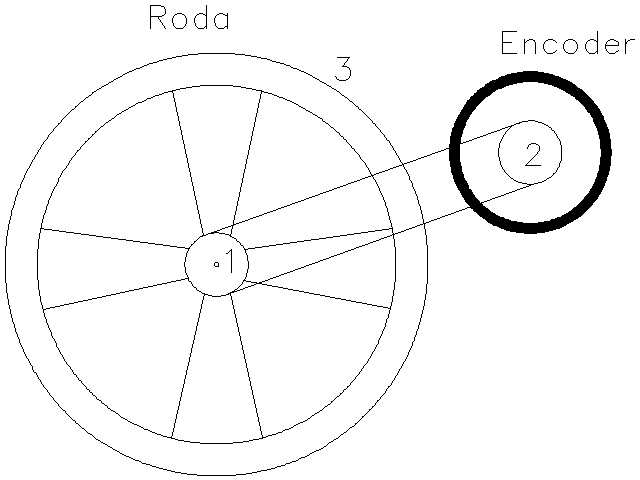
\includegraphics[width=0.5\textwidth, keepaspectratio]{./figuras/robo/roda_encoder.png}
  \caption{Representação de uma roda acoplada a um encoder.}
  \label{fig:roda_encoder}
\end{figure}

\subsection{Deslocamento de cada roda}

Um princípio importante utilizado nos cálculos é a relação entre o deslocamento $\Delta x$ ao redor de uma circunferência (de raio $R$) e a variação do ângulo $\Delta \theta$:

\begin{equation}
  \Delta x = R \cdot \Delta \theta
  \label{eq:deslocamento_circunferencia}
\end{equation}

Nos cálculos a seguir, faz-se uso do índice 1 para o eixo da roda, 2 para o eixo do encoder e 3 para a própria roda, de acordo com a figura \ref{fig:roda_encoder}. Para determinar a distância percorrida pela roda, deve-se considerar a circunferência do eixo da roda ($C_1$), a circunferência do eixo do encoder ($C_2$) e a circunferência da roda ($C_3$).

O acoplamento do eixo do encoder com o eixo da roda é feita por uma correia de borracha, e portanto considera-se que o deslocamento ($ \Delta x_1$) na superfície do eixo da roda é igual ao deslocamento ($ \Delta x_2$) na superfície do eixo do encoder. Pode-se, com isso, calcular:

\begin{eqnarray*}
   \Delta x_1 =  \Delta x_2 \rightarrow \Delta \theta_1 R_1 = \Delta \theta_2 R_2 \rightarrow \Delta \theta_1 \frac{C_1}{2 \pi} = \Delta \theta_2 \frac{C_2}{2 \pi} 
\end{eqnarray*}

\begin{equation}
  \Delta \theta_1 = \frac{C_2}{C_1} \cdot \Delta \theta_2
  \label{eq:theta1_theta2}
\end{equation}

Calculando-se a relação entre a contagem de pulsos do encoder ($E$) e o ângulo de rotação ($\Delta \theta_2$) do eixo do encoder, levando-se em conta que há uma contagem de 1800 pulsos por volta:

\begin{equation}
  \Delta \theta_2 = \frac{2 \pi}{1800} \cdot E \unit{rad}
  \label{eq:E_theta2}
\end{equation}

Substituindo-se a equação \ref{eq:E_theta2} na \ref{eq:theta1_theta2}, tem-se que:

\begin{equation}
  \Delta \theta_1 = \frac{C_2}{C_1} \frac{2 \pi}{1800} \cdot E \unit{rad}
  \label{eq:theta_1}
\end{equation}

Calculando-se a relação entre a variação do ângulo do eixo da roda ($\Delta \theta_1$) e o deslocamento da roda ($x_3$):

\begin{eqnarray*}
  \Delta \theta_1 = \Delta \theta_3 \rightarrow \Delta \theta_1 =  \Delta x_3 R_3 \rightarrow \Delta \theta_1 = \Delta x_3 \frac{C_3}{2 \pi} \rightarrow  \Delta x_3 = \Delta \theta_1 \frac{2 \pi}{C_3}
\end{eqnarray*}

Substituindo-se o valor de ($\Delta \theta_1$) da equação \ref{eq:theta_1}:

\begin{eqnarray*}
   \Delta x_3 = \frac{C_2}{C_1} \frac{2 \pi}{1800} \cdot E \cdot \frac{2 \pi}{C_3} = \frac{C_2}{C_1 C_3} \frac{(2 \pi)^2}{1800} \cdot E
\end{eqnarray*}

\begin{empheq}[box=\fbox]{equation}
   \Delta x_3 = \frac{C_2}{C_1 C_3} \frac{\pi^2}{450} \cdot E
  \label{eq:x_3}
\end{empheq}


Que é o valor do deslocamento da roda em função da contagem de pulsos do encoder. 


\subsection{Deslocamento do centro de movimento do robô}

Como já explicitado anteriormente, o centro de movimento do robô considerado é o ponto médio entre as duas rodas. As duas variáveis para determinar em cada instante de tempo são o deslocamento linear (distância absoluta percorrida) e o angular (variação do ângulo de orientação do robô). Considerando-se que em cada instante o robô descreve um movimento circular uniforme (MCU), o raio da trajerória deve ser determinado para que os cálculos de posicionamento do robô possam ser feitos. Este raio depende do deslocamento das rodas em cada instante, e é uma importante variável que será estudada na próxima subseção.

Nos cálculos que serão explicitados a seguir, utiliza-se o índice E para a roda esquerda, C para o centro de movimento do robô e D para a roda direita.

Uma relação importante a notar a princípio é que a variação do ângulo de orientação em cada instante é igual nos três pontos: E (roda esquerda), C (centro de movimento) e D (roda direita), visto que todos estão fixos em relação à carcaça do robô. Parte-se da seguinte relação fundamental, portanto:

\begin{equation}
  \Delta \theta_E = \Delta \theta_D = \Delta \theta_C
  \label{eq:relacao_fundamental_theta}
\end{equation}



\subsubsection{Raio do movimento}

Para determinar o raio ($R$) descrito pelo centro de movimento do robô em sua trajetória instantânea em MCU, usa-se os dois primeiros termos da igualdade da equação \ref{eq:relacao_fundamental_theta}:

\begin{eqnarray*}
  \Delta \theta_E = \Delta \theta_D \rightarrow \frac{\Delta x_E}{R_E} = \frac{\Delta x_D}{R_D} 
\end{eqnarray*}

Mas:
\begin{equation*}
  R_E = R + h, ~ ~ R_D = R - h
\end{equation*}

Portanto:

\begin{eqnarray*}
  \frac{\Delta x_E}{R + h} = \frac{\Delta x_D}{R - h} ~\rightarrow~ \frac{\Delta x_E}{\Delta x_D} = \frac{R + h}{R - h} ~\rightarrow~ \frac{\Delta x_E (R - h)}{\Delta x_D} = R + h 
\end{eqnarray*}
\begin{eqnarray*}
  \frac{\Delta x_E \cdot R - \Delta x_E \cdot h}{\Delta x_D} = R + h ~\rightarrow~ 
  \frac{\Delta x_E}{\Delta x_D} \cdot R - \frac{\Delta x_E}{\Delta x_D} \cdot h = R + h ~\rightarrow~ 
  \frac{\Delta x_E}{\Delta x_D} \cdot R - R = \frac{\Delta x_E}{\Delta x_D} \cdot h + h
\end{eqnarray*}
\begin{eqnarray*}
  R \left( \frac{\Delta x_E}{\Delta x_D} - 1 \right) = h \left( \frac{\Delta x_E}{\Delta x_D} + 1 \right) ~\rightarrow~
  R = h \cdot \frac{\left( \frac{\Delta x_E}{\Delta x_D} + 1 \right)}{\left( \frac{\Delta x_E}{\Delta x_D} - 1 \right)}  ~\rightarrow~
  R = h \cdot \frac{\frac{\Delta x_E + \Delta x_D}{x_D}}{\frac{\Delta x_E - \Delta x_D}{\Delta x_D}} 
\end{eqnarray*}

\begin{empheq}[box=\fbox]{equation}
  R = h \cdot \frac{\Delta x_E + \Delta x_D} {\Delta x_E - \Delta x_D}
  \label{eq:R}
\end{empheq}

Vê-se que o raio $R$ do movimento circular uniforme em cada instante depende do deslocamento de cada roda ($\Delta x_E$ e $\Delta x_D$) e da distãncia $h$ entre as rodas e o centro de movimento do robô.


\subsubsection{Deslocamento linear} 

Para calcular o deslocamento linear do centro de movimento do robô, usa-se os dois últimos termos da equação \ref{eq:relacao_fundamental_theta}. Vale ressaltar que poderiam ser escolhidos também o primeiro e o último termos, pois o resultado obtido seria idêntico. Tem-se que:

\begin{eqnarray*}
  \Delta \theta_D = \Delta \theta_C \rightarrow \frac{\Delta x_D}{R_D} = \frac{\Delta x_C}{R} 
\end{eqnarray*}

Mas:
\begin{equation*}
  R_D = R - h
\end{equation*}

Portanto:
\begin{eqnarray*}
  \frac{\Delta x_D}{R - h} = \frac{\Delta x_C}{R} ~\rightarrow~ x_D = x_C \cdot \frac{R - h}{R} 
\end{eqnarray*}

Substituindo-se o valor de $R$ da equação \ref{eq:R}:
\begin{eqnarray*}
  \Delta x_D = \Delta x_C \left[ \frac{h \cdot \frac{\Delta x_E + \Delta x_D}{\Delta x_E - \Delta x_D} - h}{h \cdot \frac{\Delta x_E + \Delta x_D}{\Delta x_E - \Delta x_D}} \right]
\end{eqnarray*}

Dividindo-se o numerador e denominador do segundo termo por $h$:
\begin{equation*}
  \Delta x_D = \Delta x_C \left[ \frac{\frac{\Delta x_E + \Delta x_D}{\Delta x_E - \Delta x_D} - 1}{\frac{\Delta x_E + \Delta x_D}{\Delta x_E - \Delta x_D}} \right]
\end{equation*}

Multiplicando-se o numerador e denominador do segundo termo por $\frac{\Delta x_E - \Delta x_D}{\Delta x_E + \Delta x_D}$:

\begin{equation*}
  \Delta x_D = \Delta x_C \left[1 - \frac{\Delta x_E - \Delta x_D}{\Delta x_E + \Delta x_D} \right] ~\rightarrow~
  \Delta x_D = \Delta x_C \left[\frac{(\Delta x_E + \Delta x_D) - (\Delta x_E - \Delta x_D)}{\Delta x_E + \Delta x_D} \right] 
\end{equation*}
\begin{equation*}
  \Delta x_D = \Delta x_C \cdot \left[ \frac{2 \Delta x_D}{\Delta x_E + \Delta x_D} \right] ~\rightarrow~
  \Delta x_C = \frac{\Delta x_D}{\left(\frac{2 \Delta x_D}{\Delta x_E + \Delta x_D} \right)}
\end{equation*}

\begin{empheq}[box=\fbox]{equation}
  \Delta x_C = \frac{\Delta x_E + \Delta x_D}{2}
  \label{eq:desloc_linear}
\end{empheq}

Notas-se que o deslocamento linear do centro de movimento do robô ($\Delta x_C$) é uma média simples dos dois deslocamentos lineares das rodas. Vê-se que ele não depende do raio de deslocamento nem da distância entre as duas rodas.


\subsubsection{Deslocamento angular}

O deslocamento angular ($\Delta \theta_c$) do centro de movimento do robô em cada instante pode ser calculado a partir do deslocamento linear e do raio do movimento circular uniforme. Usando-se a relação da equação \ref{eq:deslocamento_circunferencia}, tem-se que:


\begin{empheq}[box=\fbox]{equation}
  \Delta \theta_c = \frac{\Delta x_C}{R}
  \label{eq:desloc_angular}
\end{empheq}


Onde $\Delta x_C$ é o deslocamento linear do robô (equação \ref{eq:desloc_linear}) e $R$ é o raio do movimento circular uniforme (equação \ref{eq:R}). 

\subsubsection{Casos especiais}

Há dois casos especiais que devem ser considerados no cálculo do deslocamento (a partir dos dados dos encoders) do centro de movimento do robo. O primeiro é quando as duas rodas têm deslocamento igual ($\Delta x_E = \Delta x_D$). O raio do movimento circular (equação \ref{eq:R}) neste caso é:

\begin{equation}
  R = h \cdot \frac{\Delta x_E + \Delta x_D} {\Delta x_E - \Delta x_D} = h \cdot \frac{2 \cdot \Delta x_E}{0} \rightarrow \infty
  \label{eq:caso_especial1_R}
\end{equation}


O raio tende a infinito, o que implica que o deslocamento angular (equação \ref{eq:desloc_angular}) seja:

\begin{equation}
  \Delta \theta_c = \frac{\Delta x_C}{R} = \frac{\Delta x_C}{\infty} \rightarrow 0
  \label{eq:caso_especial1_theta}
\end{equation}

Já o deslocamento linear (equação \ref{eq:desloc_linear}) é:

\begin{equation}
  \Delta x_C = \frac{\Delta x_E + \Delta x_D}{2} = \frac{2 \Delta x_E}{2} = \Delta x_E
  \label{eq:caso_especial1_x}
\end{equation}

Isso corresponde à realidade, uma vez que quando as rodas têm deslocamentos iguais o robô está se deslocando sem fazer curvas. Não há deslocamento angular, portanto, e o deslocamento linear do centro de movimento é igual ao deslocamento de cada roda.

O segundo caso especial ocorre quando os deslocamento têm módulos iguais, porêm sentidos contrários (ou seja, $\Delta x_E = - \Delta x_D$). O raio nesse caso é:

\begin{equation}
  R = h \cdot \frac{\Delta x_E + \Delta x_D} {\Delta x_E - \Delta x_D} = h \cdot \frac{\Delta x_E - \Delta x_E}{\Delta x_E + \Delta x_E} = 0
    \label{eq:caso_especial2_R}
\end{equation}


O deslocamento linear (equação \ref{eq:desloc_linear}) é:

\begin{equation}
  \Delta x_C = \frac{\Delta x_E + \Delta x_D}{2} = \frac{\Delta x_E - \Delta x_E}{2} = 0
  \label{eq:caso_especial2_x}
\end{equation}

Esse valor corresponde à realidade, pois quando as rodas se deslocam em sentidos contários, e na mesma quantidade, o centro de movimento do robô não se desloca linearmente, mas apenas muda seu ângulo.
Usando-se a equação \ref{eq:desloc_angular}, tenta-se calcular o valor do deslocamento angular:

\begin{equation}
  \Delta \theta_c = \frac{\Delta x_C}{R} = \frac{0}{0}
  \label{eq:caso_especial2_theta}
\end{equation}

O valor obtido é indeterminado quando usa-se essa equação. Porém, analisando-se a natureza deste caso especial, pode ser notado que há um movimento circular cujo centro é o ponto médio entre as rodas (que é o centro de movimento do robô). O raio do MCU é a distância $h$ entre uma roda e o centro do robô, e o deslocamento ao longo da circunferência é o deslocamento de qualquer uma uma das rodas. Portanto, a equação \ref{eq:deslocamento_circunferencia} pode ser utilizada, isolando-se a variável $\theta$, para determinar o deslocamento angular do robô:

\begin{equation}
  \Delta \theta_c = \frac{\Delta x_E}{h}
  \label{eq:caso_especial2_theta2}
\end{equation}


\subsubsection{Velocidade e aceleraçao}

A velocidade e aceleração lineares do centro de movimento do robô podem ser calculadas por derivação numérica do deslocamento e velocidade em cada intervalo de tempo, considerando-se a velocidade e aceleração anteriores. Em cada intervalo discreto $n$:

\begin{equation}
  v_{c (n)} = \frac{x_{c (n)} - x_{c (n-1)}}{t_{(n)} - t_{(n-1)}}
  \label{eq:velocidade}
\end{equation}

\begin{equation}
  a_{c (n)} = \frac{v_{c (n)} - v_{c (n-1)}}{t_{(n)} - t_{(n-1)}}
  \label{eq:velocidade}
\end{equation}


A velocidade e aceleração angulares podem ser também obtidas por derivação numérica, considerando-se que o raio do movimento circular uniforme do robô é constante dentro do intervalo considerado. Em cada intervalo discreto $n$:

\begin{equation}
  \omega_{c (n)} = \frac{\theta_{c (n)} - \theta_{c (n-1)}}{t_{(n)} - t_{(n-1)}}
  \label{eq:velocidade}
\end{equation}

\begin{equation}
  \alpha_{c (n)} = \frac{\omega_{c (n)} - \omega_{c (n-1)}}{t_{(n)} - t_{(n-1)}}
  \label{eq:velocidade}
\end{equation}


\section{Acelerômetro e giroscópio}
\label{sec:teoria_acel_giro}

O acelerômetro e o giroscópio são utilizados para aumentar a confiabilidade dos dados de deslocamento do robô em caso de escorregamento das rodas.



Como definido na seção \ref{sec:codificacao_mensagens}, é recebido um valor de 2 bytes para cada eixo do acelerômetro. A faixa de funcionamento do acelerômetro está configurada em $-+2g$, logo a sensibilidade pelo \textit{datasheet} é de $16384 LSB/g$. Portanto, o valor de aceleração pode ser obtido pela fórmula:

\begin{equation}
  a = \frac{valorMedido}{16384} \cdot g \unit{m/s^2}
  \label{eq:acel}
\end{equation}

Onde g é a aceleração da gravidade ($9,80665 \unit{m/s^2}$). 

Para cada eixo do giroscópio, também e obtido um valor de 2 bytes. A faixa de funcionamento do giroscópio está configurada em $-+250$ graus/s, logo a sensibilidade pelo \textit{datasheet} é de 131 LSB/(graus/s). Portanto, o valor de velocidade angular pode ser obtida pela fórmula:

\begin{equation}
  \omega = \frac{valorMedido}{131} \unit{graus/s} = \frac{\pi}{180} \cdot \frac{valorMedido}{131} \unit{rad/s}
  \label{eq:giro}
\end{equation}


A princípio, apenas o eixo X do acelerômetro (voltado para a frente do robô) e o eixo Z do giroscópio (posicionado no sentido baixo/cima) serão utilizados para mapeamento, visto que poderão ser comparados facilmente com os dados obtidos pelos encoders. A ideia é posicioná-los no centro de movimento do robô (ponto médio entre as rodas) para que a comparação seja feita.

A velocidade e deslocamento lineares podem ser obtidos por integração numérica da aceleração linear em cada intervalo discreto $n$:

\begin{equation}
  v_{(n)} = v_{(n - 1)} + a_{(n)} \cdot (t_{(n)} - t_{(n-1)})
  \label{eq:v_acel}
\end{equation}

\begin{equation}
  \Delta x_{(n)} = \Delta x_{(n - 1)} + v_{(n)} \cdot (t_{(n)} - t_{(n-1)})
  \label{eq:v_acel}
\end{equation}

O deslocamento angular pode ser obtido por integração numérica da velocidade angular em cada intervalo discreto $n$:

\begin{equation}
  \Delta \theta_{(n)} = \Delta \theta_{(n - 1)} + \omega_{(n)} \cdot (t_{(n)} - t_{(n-1)})
  \label{eq:v_acel}
\end{equation}



\section{Sensores infra-vermelhos}

Para obter a posição em que cada obstáculo detectado está no mapa, primeiramente deve-se obter a distância detectada por cada sensor infra-vermelho. Como explicitado em \cite{bellator_2012}, o valor recebido em 1 byte do sensor pode ser convertido para a distãncia em centímetros pela fórmula (obtida por interpolação polinomial):

\begin{equation}
  y = 3,6404 \cdot 10^{-7} x^3 - 2,4435 \cdot 10^{-4} x^3 + 6,0732 \cdot 10^{-2} x^2 - 6,8962 x + 339,361
  \label{eq:IR_dist}
\end{equation}


Sendo $\overrightarrow{P_C}$ o vetor que sai da origem e vai até o centro de movimento do robô, $\overrightarrow{P_1}$ o vetor que vai do centro do robô até o sensor, e $\overrightarrow{P_2}$ o vetor que vai do sensor até o ponto do obstáculo detectado, faz-se a seguinte soma vetorial para encontrar o vetor $\overrightarrow{P}$, que é o ponto do obstáculo detectado no mapa:

\begin{equation}
  \overrightarrow{P} = \overrightarrow{P_C} + \overrightarrow{P_1} + \overrightarrow{P_2}
  \label{eq:IR_vector}
\end{equation}


O vetor $\overrightarrow{P_C}$ é determinado facilmente, pois é a última posição do robô. $\overrightarrow{P_1}$ é o vetor da posição do sensor relativa ao centro (informação obtida das configurações iniciais do robô), rotacionado pelo ângulo em que o robô está na última posição. $\overrightarrow{P_2}$ pode ser obtido criando-se um vetor com magnitude igual à distância detectada pelo sensor, e ângulo igual a: ângulo relativo do sensor no robô (informação obtida das configurações iniciais) somado com o ângulo em que o robô está na última posição.

\section{Algoritmo de posicionamento}

O algoritmo proposto para utilização dos vários sensores (encoder, acelerômetro e giroscópio) está exposto abaixo. Para cada amostra dos sensores recebida, o algoritmo efetua os seguintes passos:

\begin{enumerate}
      \item A partir das leituras dos encoders, calcular deslocamento linear ($x_e$, em metros) e angular ($\theta$, em $rad$) do centro de movimento do robô.
      \item Derivar duas vezes o deslocamento linear $x_e$ para obter aceleração linear ($a_e$, em $m/s^2$). Derivar uma vez o deslocamento angular $\theta_e$ para obter a velocidade angular ($\omega_e$, em $rad/s$).
      \item Comparar aceleração linear $a_e$ e velocidade angular $\omega_e$, obtidas com os encoders, com as leituras do acelerômetro ($a_a$) e giroscópio ($\omega_g$). Caso a diferença das acelerações passe de um limite (determinado experimentalmente), é provável que um escorregamento de rodas tenha ocorrido.
      \item Baseado na comparação anterior, especificar pesos para a aceleração linear (encoders \textit{vs.} acelerômetro) e velocidade angular (encoders \textit{vs.} giroscópio), dando mais prioridade ao acelerômetro e giroscópio caso escorregamentos sejam detectados.
      \item Integrar duas vezes a aceleração linear final para obter o deslocamento linear do robô. Integrar uma vez a velocidade angular final para obter o deslocamento angular do robô.
\end{enumerate}


O acelerômetro e giroscópio entram em ação quando diferenças muito grandes entre os dados destes e dos encoders forem detectadas. A diferença limite para que essa detecção ocorra é determinada experimentalmente.

